\chapter{Actors}
\label{ch:actors}

Actors specify a role played by a user or a system for the purposes of a clearer definition.
In this chapter, we will outline the actors in our system.

\begin{landscape}
	\topskip0pt
	\section{Big Picture}
	\begin{figure}[H]
		\begin{center}
			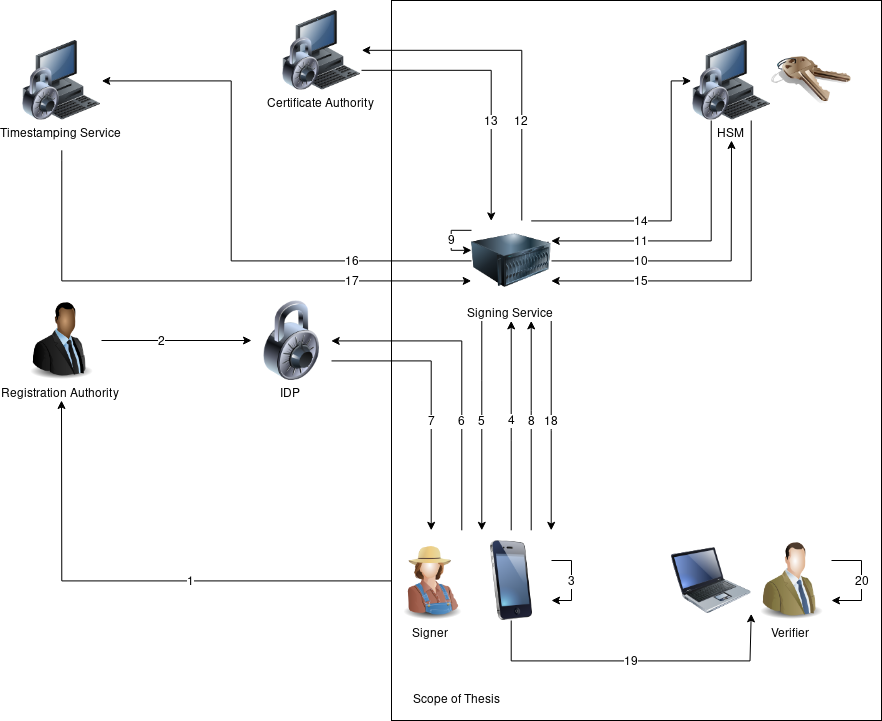
\includegraphics[scale=0.6]{images/BigPicture.png}
			\caption{Big Picture}
			\label{fig:bigpicture}
		\end{center}
	\end{figure}
\end{landscape}

\subsubsection{Steps}
\begin{enumerate}
	\item Registration of identity with RA (Authenticator)
	\item Propagate identity to IDP (Identifier)
	\item Generate document hash
	\item Send hash to signing service
	\item Receive OIDC redirect to IDP
	\item Login to IDP
	\item Receive ID token
	\item Send ID token to signing service
	\item Verify ID token
	\item Request signing key CSR from HSM
	\item Receive CSR
	\item Send CSR to CA
	\item Receive signed Certificate
	\item Request signature from HSM
	\item Receive signature
	\item Request timestamp from TSS
	\item Receive timestamp
	\item Send signature to signer
	\item Send document and signature to Verifier/Receiver
	\item Verify document and signature
\end{enumerate}


\section{The Signer}
\label{sec:actorsigner}
The Signer is the person who wishes to have the signing server sign a document in their name.
For example, a medical professional issuing a prescription for medication to a patient.

\section{The Verifier}
\label{sec:actorverifier}
The Verifier is the person who wishes to verify the integrity and authorship of a document.
For example, the pharmacist whom the patient gives the prescription to (as previously authored and signed by The Signer as specified in section~\ref{sec:actorsigner}) in order to purchase the medication prescribed by the medical professional.

\section{The Authenticator}
\label{sec:actorauthenticator}
The Authenticator is the system who authenticates The Signer as specified in section~\ref{sec:actorsigner}.
In \gls{NIST} terminology~\cite{nistdigitalidentityguidelines}, this is the entity establishing the \gls{IAL}.
In order for The Authenticator to be able to authenticate The Signer,
they must have been registered with The Authenticator by The Identifier as specified in section~\ref{sec:authoridentifier}.

\section{The Identifier}
\label{sec:authoridentifier}
The Identifier is the system or person who asserts the identity of The Signer.
In order for the signing service to issue qualified signatures as defined by relevant Swiss legislation~\cite{zertes} and Swiss Federal Council regulations~\cite{vzertes},
the identity must be proven in-person using a government-issued photographic identification document such as a passport.

\section{The Signing Service}
\label{sec:signingservice}
The Signing Service is the system who actually creates the signatures on behalf of the user.
It generates the signing keys and requests the \gls{CA}~\ref{sec:ca} to sign them.

\section{The Certificate Authority}
\label{sec:ca}
The \gls{CA} is the system who signs the signing keys generated by the Signing Service~\ref{sec:signingservice}.
